\section{Evaluation}
\label{section:evaluation}

In this chapter the system designed in Chapter~\ref{section:design_and_implementation} and implemented in Chapter~\ref{sec:implementation_and_deployment_details} will be evaluated. First the methodology of this evaluation will be documented and then the results are demonstrated.

The evaluation will refer to a particular use case presented in Section~\ref{subsec:implementation_details}. The evaluation for the general SSI with IoT architecture presented in Section~\ref{subsec:architecture_for_ssi_with_iot} will be discussed at the end of this chapter. 

\subsection{Methodology}
\label{subsec:methodology}

% In order to evaluate a system that relies heavily on open-source software and whether the requirements are satisfied with the assumptions that were made, the evaluation does not regard benchmarking the actual proof-of-concept system, but rather assessing if the main components used can comply with the requirements listed in Chapter~\ref{sec:requirement_elicitation}.

The evaluation will be split into three distinct steps:

\begin{itemize}
    \item Benchmark the "Hyperledger Indy Network" and "Hyperledger Aries Cloud Agent - Python" in order to assess performance-, scalability- and availability-related NFRs;
    \item Qualitative evaluation of the proposed solution from domain experts;
    \item Cross-check requirements against the decisions taken throughout the project (and evaluation results).
\end{itemize}

\paragraph{Benchmark "Hyperledger Indy Network" and "Hyperledger Aries Cloud Agent - Python"}

This part of the evaluation will be made possible with the help of the development team of Hyperledger Indy, since performance and scalability tests were already made to the network. The results from these tests will be presented to validate the Non-Functional Requirements of the system.

Given that the agents are a core part of the system, being able to know the time they take to perform their tasks is imperative to know if these can be used at scale.

\paragraph{Qualitative evaluation from domain experts}

In order to measure the validity of the new system, and whether it can actually be considered an improvement to the current implementation (dissected in Section~\ref{subsec:case_description}), a qualitative assessment from domain experts is a vital part of understanding whether some assumptions are valid, feasible or impossible. 
This evaluation process consisted of:
\begin{itemize}
    \item Gathering contacts from various domain-specific experts that are related to the targeted use case (Energy, Blockchain, Self-Sovereign Identity).
    \item Inviting contacts to participate in the evaluation process, by having them sign up via a Google Forms with preliminary assessment questions, to profile the participants.
    \item Recording a presentation of the project with a small demo to send to the interested participants.
    \item Sending the interested evaluators the recorded presentation and demo, together with a Google Forms to assess their perspective on certain aspects of the system. 
\end{itemize}

\paragraph{Cross-check requirements} 

For this part of the evaluation, each requirement will be analyzed and discussed, to understand whether in the novel architecture of the system that given requirement is (partially) met, or not.


\subsection{Benchmark "Hyperledger Indy Network" and "Hyperledger Aries Cloud Agent - Python"}
\label{subsec:benchmark_hyperledger_indy_and_aries}

\paragraph{Hyperledger Indy Network evaluation}

As mentioned before, assessing the capability of the network that is the backbone of the proposed solution is a major part of understanding if it can handle the proposed use case requirements. Investigating performance tests made to the network landed on an issue on the Indy's JIRA repository. 
Issue \textbf{INDY-1343 - Prove production stability of an Indy network}\footnote{\url{https://jira.hyperledger.org/browse/INDY-1343}} arose from the following need: \textit{"Before encouraging people to use the Sovrin network for live loads, we need to prove that it will be stable under conditions similar to production use."} 
Sovrin's name has been highlighted previously in the Related Work chapter (Section~\ref{subsubsec:hyperledger_indy_sovrin}), and corresponds to the production level network created by the Sovrin Foundation.

The tests had mixed conclusions, with certain scenarios underperforming while others achieving the expected TPS throughput. After these tests, three more issues were lifted on the project's JIRA repository related to testing the performance of the network, INDY-1388\footnote{\url{https://jira.hyperledger.org/browse/INDY-1388}}, INDY-1607\footnote{\url{https://jira.hyperledger.org/browse/INDY-1607}} and INDY-2214\footnote{\url{https://jira.hyperledger.org/browse/INDY-2214}}. Table~\ref{tab:benchmarks_indy} contains information on the issues regarding network stability and their current status. It is worth noting that the latest issue (INDY-2214) has yet to be resolved, since December 2019. A detailed description of the tests can be found in a Google Sheets shared by the development team, that highlights their findings\footnote{\url{https://docs.google.com/spreadsheets/d/1DTjDsLSysFBiKU-9z4-IzunJk4wEy44hE_PGZYxnN_8/edit\#gid=1813415708}} (Available on 13th June 2021).

\begin{table}[t]
    \centering
    \begin{tabular}{|ccc|}
    \hline
        Issue \# & Title & Status \\
        \hline
        INDY-1343 & Prove production stability of an Indy network & \greencheck \\
        INDY-1388 & Prove stability under a DOS of an Indy network & \greencheck \\
        INDY-1607 & Proof of stability under load & \greencheck \\ 
        INDY-2214 & Repeat: Prove production stability of an Indy network & - \\
        \hline
    \end{tabular}
    \caption{Issues on Indy's JIRA Repository related to benchmarking the network}
    \label{tab:benchmarks_indy}
\end{table}

Although arguably the JIRA or the project's GitHub repositories are usually the best source of information regarding benchmarking tests, the best source to validate the current state of the Hyperledger Indy network comes directly from the Sovrin's foundation network status dashboard\footnote{\url{https://sovrin.org/ssi-metrics-dashboards/}}. Figure~\ref{fig:sovrin_metrics} demonstrates the network status from 12th June 2020 to 12th June 2021, regarding various metrics. The most relevant information regards the read and write availability, that achieves an outstanding \textbf{99.999\% read and write availability}.

\begin{figure}[!htb]
    \centering
    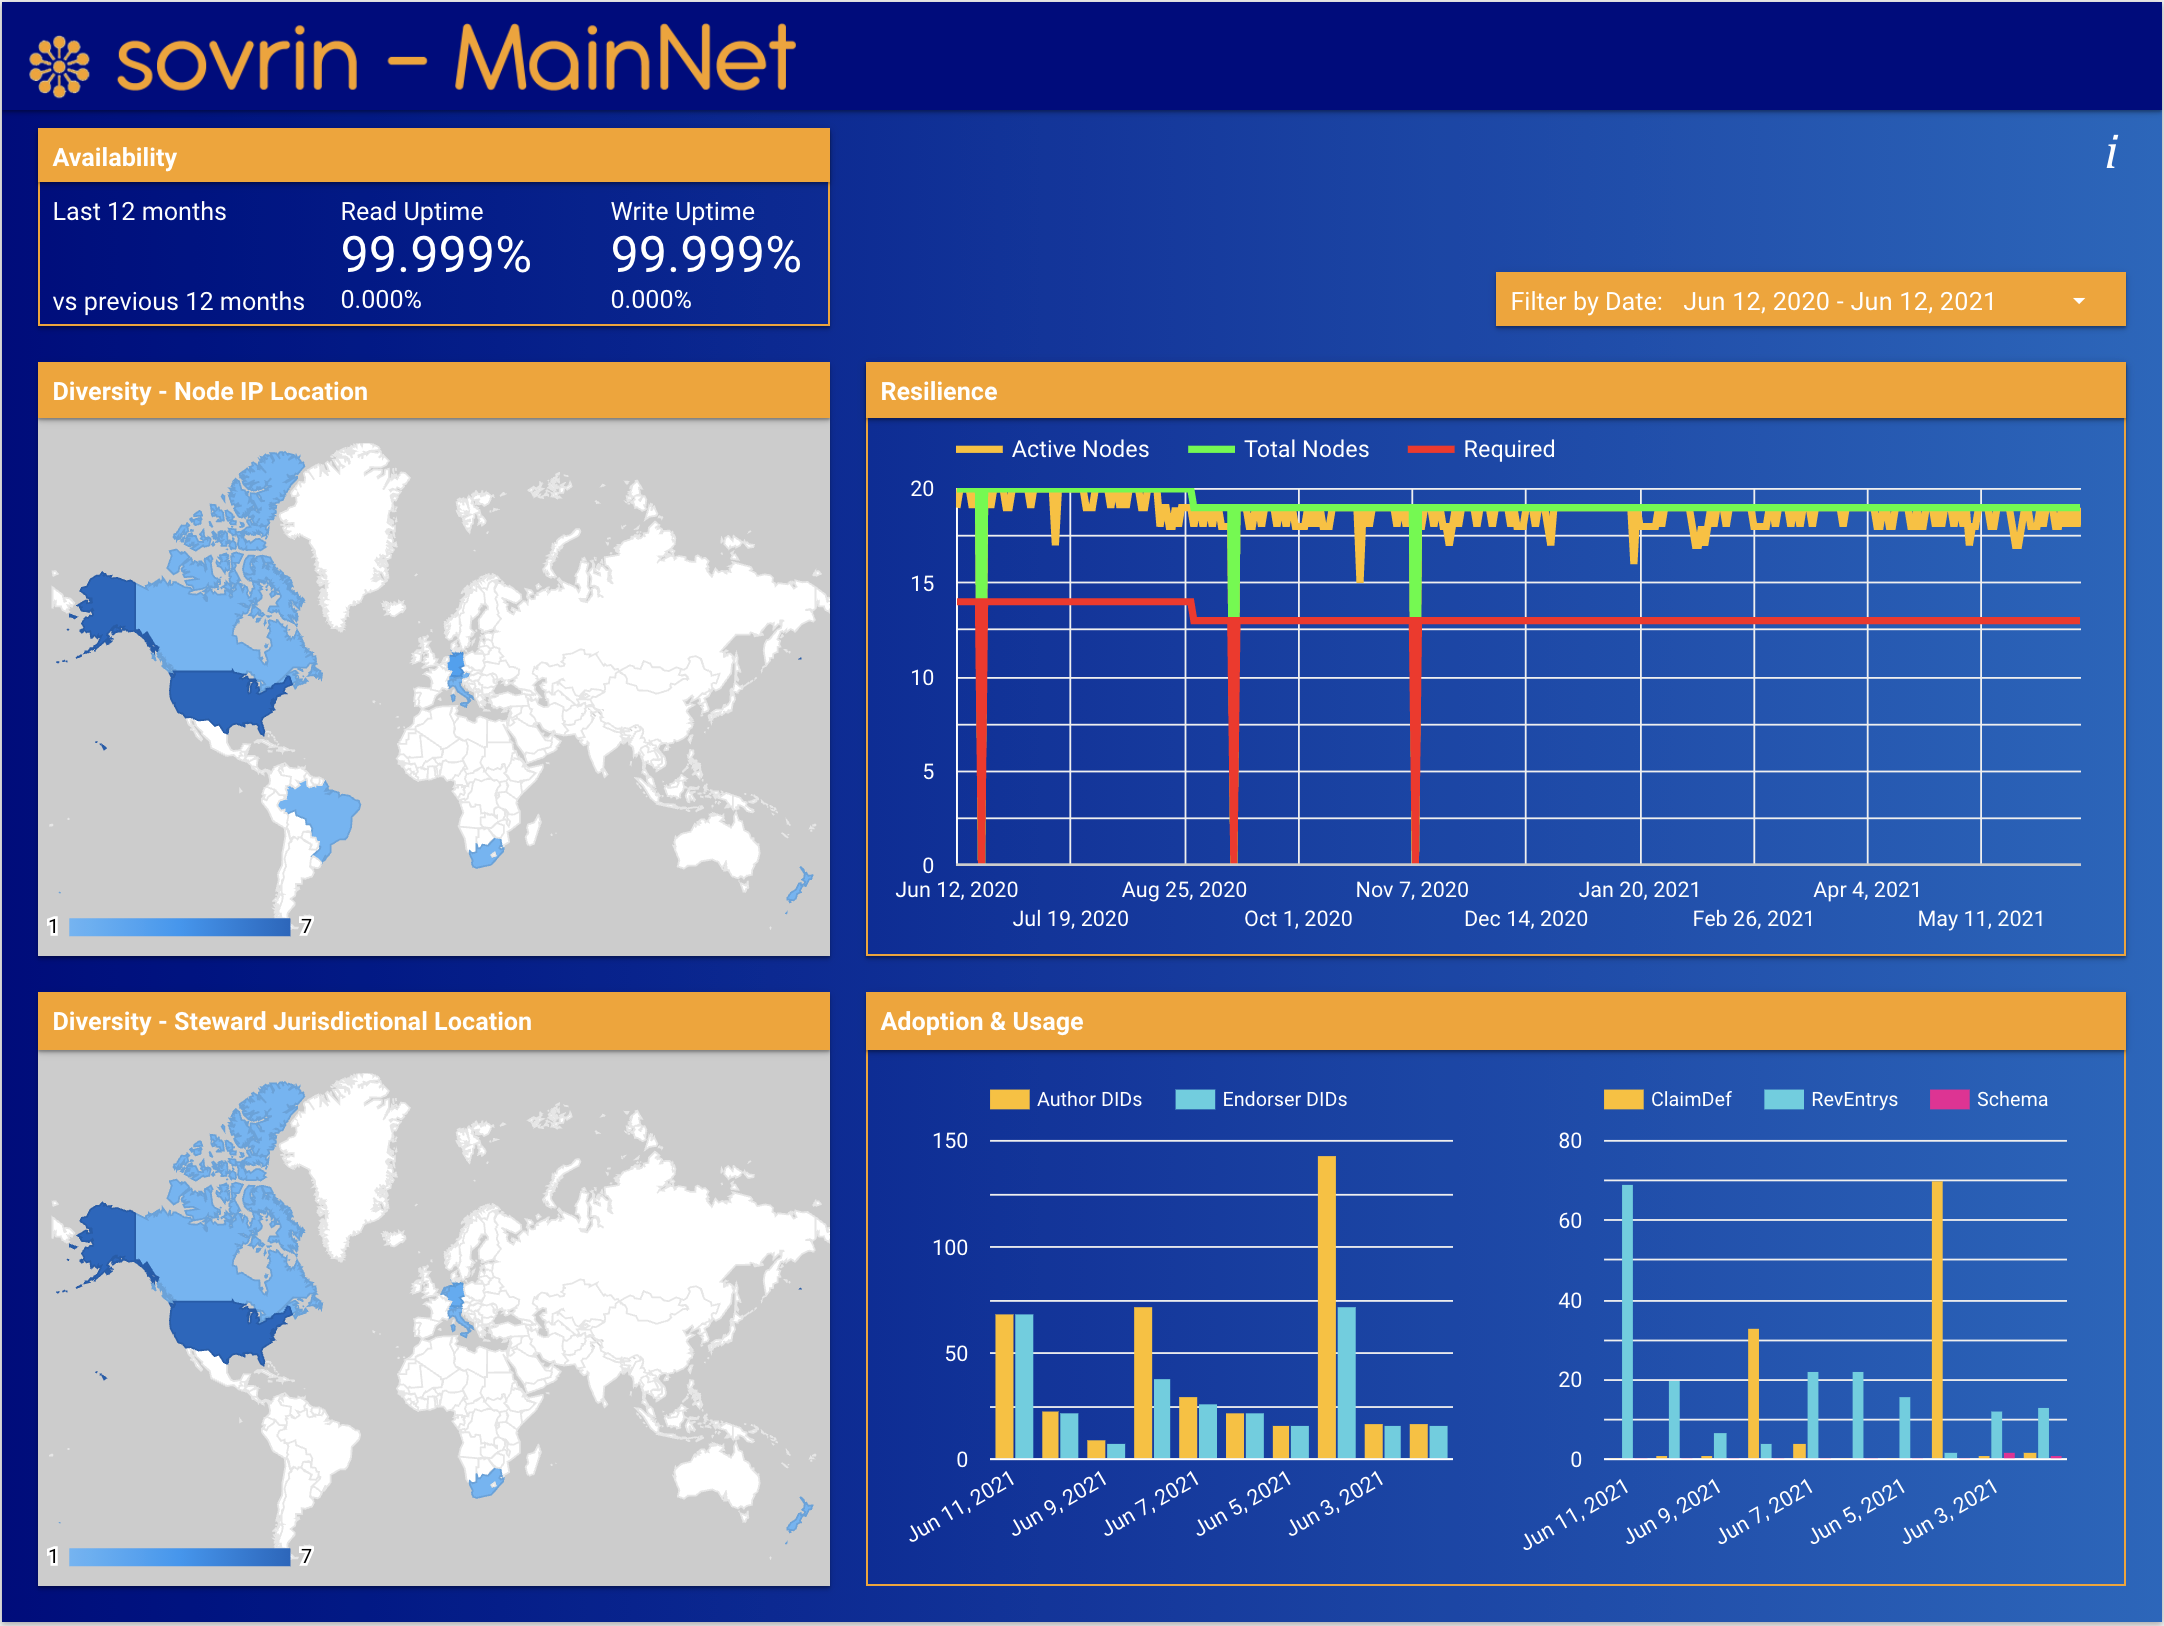
\includegraphics[width=0.8\linewidth]{images/sovrin_metrics.png}
    \caption{Sovrin Network (Hyperledger Indy nodes) metrics from 12 June 2020 to 12 June 2021}
    \label{fig:sovrin_metrics}
\end{figure}

\paragraph{Hyperledger Aries Cloud Agent - Python evaluation}

In order to assess the performance of the agent implementation, two different methods were used: Use the performance benchmark tests provided by the development team; and measure the times when conducting actions with the agents in the proof-of-concept implementation.

For the first, in the original Aries Cloud Agent - Python repository the developers included a basic \textit{performance.py} script that deploys two agents, and has one issue a predefined number of credentials to the other. These benchmarks are therefore a good indication of the times taken to issue credentials from one agent to another, and can vary depending on whether there is mediation between the two agents or not, and also if the credentials are revoked after they are issued.
This latter also indicates the feasibility to revoke credentials, something that was not explored in-depth with the proof-of-concept. 
For the second set of benchmarks to the agent implementation, the interactions of the agents will be timed manually to assess the performance requirements. The commands used to execute each of the runs, as well as more details extracted from the runs are listed in Appendix~\ref{app:benchmark_runs}.
In this appendix the computer specifications are also listed for reference. 

Looking at the results found in Table~\ref{tab:overview_of_different_attempts}, it is possible to see that an ACA-Py agent is able to issue credentials to another agent in an acceptable time, averaging 0.23s in three of the runs and 0.26s in the last. Note that these results are limited by the fact that the agents are running in the same piece of hardware, which may lead to an improvement in the times. Still, the results are 10 times faster than the time of interactions of the current system's validation periods, as listed in \textbf{Requirement NFR-2.4} - \textit{The process of validation the client's credentials should not take longer than the original method (designed for 2 seconds, with the worst case scenario being 30 seconds)}. For this reason, it is possible that the times may increase in a production environment, but not exceeding the optimal range of values.

\begin{table}[t]
    \centering
    \begin{tabular}{|ccccc|}
    \hline
        Run \# & Revocation & Mediation & Count & Average Credential Times \\
        \hline
        1 & \redcheckk & \greencheck & 1000 & 0.23s \\
        2 & \greencheck & \redcheckk & 1000 & 0.23s \\
        3 & \redcheckk & \redcheckk & 1000 & 0.23s \\
        4 & \greencheck & \greencheck & 1000 & 0.26s \\
        \hline
    \end{tabular}
    \caption{Overview of the different attempts}
    \label{tab:overview_of_different_attempts}
\end{table}

Besides these tests made to the credential issuance process, the actions needed for the charging process were also manually timed. 
When performing the charging process, the "Request Proofs" action from the EV Owner took on average less than 2 seconds. Note that this step occurs between an ACA-Py agent and a Trinsic Wallet agent.
For the process of the "Request EV Credentials" from the EV agent, this process also takes less than 2 seconds on average. This process involves the CS agent sending the request for the proof, the EV agent generating the proof, sending it back to the CS agent and then it being verified. 
At last, the "Issue Receipt Credential" process from the CS to the EV Owner's Trinsic Wallet agent also takes on average less than 2 seconds, but depends on the internet signal at the time of receiving the credential proposal on the Trinsic Wallet App dashboard.

\subsection{Qualitative Evaluation from domain experts}
\label{subsec:qualitative_evaluatin_from_domain_experts}

In this section the results from the evaluation provided by the domain experts will be presented to extract results that can validate the requirements.

\subsubsection{Preliminary Form Results}
\label{subsubsec:preliminary_form}

In the preliminary form shared with potential participants to the evaluation, the questions mostly related to profile questions, to understand the area expertise of the evaluators and how well they are aware of the charging process of EVs.
A total of six (6) people responded to the form, confirming their willingness to evaluate the proposed solution. Note that some of the participants had expertise in more than one area as demonstrated by Table~\ref{tab:expertise_of_evaluators}.

\begin{table}[!htb]
    \centering
    \begin{tabular}{|cc|}
    \hline
    Field of Expertise & Count \\
    \hline
    Blockchain & 4 \\
    Energy & 3 \\
    Self-Sovereign Identity & 1 \\
    Architecture & 1 \\
    EV Automotive & 1 \\
    \hline
    \end{tabular}
    \caption{Expertise of the Evaluators}
    \label{tab:expertise_of_evaluators}
\end{table}

From the six respondents, the follow data was extracted:

\begin{itemize}
    \item 3 out of 6 responded to be able to "teach someone else" about blockchain.
    \item 2 out of 6 responded to be able to "teach someone else" about Self-Sovereign Identity.
    \item None of the respondents own an EV, but more than half (4) of them are knowledged in the process of charging an EV. Out of those 4 people, 4 are aware of (most of) the parties in the process, 3 know how to charge an EV, and only 2 of them are aware of the current payment model.
\end{itemize}

\subsubsection{Results from experts' evaluation of system}
\label{subsubsec:results_from_experts_evaluation_of_system}

After gathering the profiles of the six evaluators, a video containing a pre-recorded slide presentation explaining the project was shared with the latters. In this video it was included part of the proof-of-concept's demonstration of how an EV Owner is able to charge its EV making use of Verifiable Credentials to attest the claims explained in the flow present in Section~\ref{paragraph:charging_and_billing_flow_with_ssi}.

This expert evaluation was mostly used to assess the usability requirements as well as the business value of the novel architecture. From the six (6) evaluators that agreed to answer the preliminary form, the following results arose:

When asked to prioritize "Ease of Use", "Data Privacy", "Cost Transparency", "Availability" and "Integration with Mobile Applications" in  an EV Charging Network from the least important (1) to the most important (5), these were the results:

\begin{itemize}
    \item Availability and Cost Transparency both obtained 23 points, making these two the most prioritized quality attributes;
    \item Ease of Use obtained 22 points, close to the first two quality attributes.
    \item Data Privacy and Integration with Mobile Applications scored 14 and 8 points, respectively, demonstrating that these two are not the highest priority for the evaluators.
\end{itemize}

The questions below constitute the questionnaire made to the evaluators. Each of them was given an ID.

\begin{itemize}
    \item \#1 - \textit{How understandable is the presented solution, from a user and business perspective?}
    \item \#2 - \textit{How do you think the solution compares with the current implementation of the network?}
    \item \#3 - \textit{With this solution, would you feel confident your personal data is protected?}
    \item \#4 - \textit{With this solution, would you consider the process of charging the vehicle more transparent?}
    \item \#5 - \textit{Do you consider the employed payment model user-friendly?}
    \item \#6 - \textit{Which feature(s) from this solution did you appreciate the most?}
    \item \#7 - \textit{Which feature(s) would you like to see added to this solution?}
    \item \#8 - \textit{Do you have any other comments on the presented solution?}
\end{itemize}


From the aforementioned questions, the more relevant finding were:

\begin{itemize}
    \item 4 out of 6 believe that the solution is "Very easy to understand" from a user perspective while 3 out of 6 thought the same from a business perspective.
    \item 4 out of 6 believe that the new solution is much better than the current implementation of the network.
    \item At least 6 out of 6 "Agree" with question \#3, with 3 of them selecting "Strongly Agree".
    \item The same results from question \#3 were obtained for question \#4.
    \item 5 out of 6 "Agree" to question \#5 regarding the user-friendliness of the payment model.
    \item The feature with the most appreciation was the "Added more transparency with the addition of the kWh price" feature, with 4 evaluators selecting that option for question \#6. 3 evaluators also enjoyed the "Removal of Login", 2 selected "Added Vehicle and Owner verification for extra security" and 1 liked the "Removal of external party - Maximising revenue" feature. None of the evaluators saw great value in the "Added receipt-credential to the end of the transaction".
\end{itemize}

For question \#7 regarding possible future features to add, the comments made by the evaluators are found below.

\begin{spverbatim}
"I know that right now there is a solution to have multiple suppliers per charge poll and users can charge their cars in different location. So an approach is based on you credentials and your supplier contract, this should be easy to identify and get a message saying you are now charging your car with supplier A in this rate."
    
"Using a unique vehicle identity in the process might give away the owner or driver, compromising privacy. Zero-knowledge might help alleviate that iff the vehicle ID is not anyway shared with the charging station."

"Include price options in case you are not in a hurry to charge and the network can use the optimal moment to charge, although that is not really related to the SSI part."

"try to remove as much steps in the user interaction as possible."

\end{spverbatim}

For question \#8 regarding additional comments or the overall appraisal of the system, the comments made by the evaluators are found below.

\begin{spverbatim}
"The overall process is well thought-out and nicely implemented."

"I understand the value of SSI for identifying myself as the owner or the car and the one charging it, however what is the benefit of sharing the receipt as a VC? That is also shared with the energy supplier, right? Or is that to resolve a dispute on the invoice in case the supplier charges you more? Or do you see scenario's where I would need to share that with some other party?"

"Excelent demo showing the way forward for EV charging"

"Although data privacy is not a major requirement for me, I would still prefer to have something that protects me as per your solution than what is currently in the market today"

"Need to think about multiple users of a single vehicle and also Fleet driver use case."

\end{spverbatim}

The overall assessment of this evaluation method allowed to understand how domain experts in the area perceive the system, which in turn granted good prospects to fulfill the necessary requirements. All evaluators provided valuable feedback and the consensus was that the solution is an improvement to the previous iteration, providing more transparency to the system and improved the user's experience with the system. The privacy limitations regarded in the comments will be addressed at a later stage, when cross-checking the requirements.


\subsection{Cross-check requirements}
\label{subsec:cross-check-requirements}

In this section, the requirements listed in Section~\ref{subsec:list_of_requirements_and_decisions} will be evaluated, and a link to the respective motivation and rationales is traced to a more detailed description that will be found in Appendix~\ref{app:requirement_evaluation}. These motivations reflect whether the specific requirement is satisfied or not using the decisions taken across the document (from technological, architectural or assumptions). For more information regarding the assessment of each requirement, the appendix contains all the necessary information for that purpose. Despite that, a few of the most important requirements will be discussed to highlight the most important decisions.

For both upcoming sections, a table has been made containing a mapping between the RequirementID, the priority of the requirement, the approval status and a link to the respective detailed table on the appendix. 
Below it is possible to find a legend for the different status symbols and their meaning.

\begin{itemize}
    \item \greencheck : Requirement fulfilled
    \item \textbf{-} : Needs further investigation or inconclusive
    \item \redcheckk : Requirement not fulfilled
\end{itemize}

\subsubsection{Functional Requirements}
\label{subsubsec:evaluation_functional_requirements}

Table~\ref{tab:full_requirements_evaluation_table(FR)} contains the aforementioned table, and it is possible to observe that regarding the Functional Requirements, almost all of the requirements were met, with the exception of one whose priority is a "Could have" and another which is prioritized as a "Must have".

Starting with the most important requirements that were fulfilled, the ones that add more value to the novel system and eliminate the liabilities presented in the case description in Section~\ref{subsubsec:current_liabities} are \ref{evaluation:FR-1.2}, \ref{evaluation:FR-1.4}, \ref{evaluation:FR-3.1} and \ref{evaluation:FR-5.1}. Requirement~\ref{evaluation:FR-1.2} reflects on the fact that now the EV Owner is presented with a kWh rate before the charging session takes place, allowing the owner to decide whether to charge the EV at that time. This price is dependant on the contracted eMSP company, given that different companies might obtain better contracts with the CPOs and provide better prices for their clients. Requirement~\ref{evaluation:FR-1.4}'s fulfillment provides a way for the EV Owners to obtain a receipt at the end of each charging session, in the form of a Verifiable Credential. This allows the client to obtain proof of that transaction, with information regarding the full price of the charging session, providing more transparency to the latter. Requirement~\ref{evaluation:FR-3.1} addresses the fact that the EV Owner now is forced to prove ownership of the EV in order to charge the vehicle, giving the system an extra layer of security, preventing thieves from charging stolen EVs. Requirement~\ref{evaluation:FR-5.1} concerns matters of privacy, since Personally Identifiable Information (PII) should not be written to any publicly accessible repository, to comply with current privacy regulations. This matter is fulfilled with the current SSI implementation, that only writes credentials and private DIDs (PII) to the entity's wallet and not in the DLT itself, complying with this requirement. For the requirements that were not addressed by the system (\ref{evaluation:FR-3.3} and \ref{evaluation:FR-6.1}), the rationale behind their absence from the system will be detailed when explaining the limitations of the system in Section~\ref{subsubsec:limitations}.

\begin{longtable}{|p{.15\textwidth}p{.1\textwidth}p{0.05\textwidth}p{.2\textwidth}|}
    \hline
    \textbf{ID} & \textbf{Priority} & \textbf{Status} & \textbf{Appendix}\\
    \hline
    \hline
   \textbf{FR-1.1} & Must & \greencheck & \ref{evaluation:FR-1.1} \\
   \textbf{FR-1.2} & Should & \greencheck & \ref{evaluation:FR-1.2}\\
   \textbf{FR-1.3} & Must & \greencheck & \ref{evaluation:FR-1.3}\\
    \textbf{FR-1.4} & Could & \greencheck & \ref{evaluation:FR-1.4} \\
    \hline
    \textbf{FR-2.1} & Must & \greencheck & \ref{evaluation:FR-2.1} \\
    \textbf{FR-2.2} & Must & \greencheck & \ref{evaluation:FR-2.2} \\
    \textbf{FR-2.3} & Must & \greencheck & \ref{evaluation:FR-2.3} \\
    \hline
    \textbf{FR-3.1} & Should & \greencheck & \ref{evaluation:FR-3.1}  \\
    \textbf{FR-3.2} & Must & \greencheck & \ref{evaluation:FR-3.2}   \\
    \textbf{FR-3.3} & Could & \redcheckk & \ref{evaluation:FR-3.3}  \\
    \textbf{FR-3.4}& Should & \greencheck &  \ref{evaluation:FR-3.4} \\
    \hline
    \textbf{FR-4.1} & Must & \greencheck &  \ref{evaluation:FR-4.1} \\
    \hline
    \textbf{FR-5.1} & Must & \greencheck &  \ref{evaluation:FR-5.1} \\
    \textbf{FR-5.2} & Must & \greencheck &  \ref{evaluation:FR-5.2} \\
    \hline
    \textbf{FR-6.1} & Must & \redcheckk & \ref{evaluation:FR-6.1} \\
    \hline
    \caption{Requirements Verification (Functional Requirements)}
    \label{tab:full_requirements_evaluation_table(FR)}
\end{longtable}

\subsubsection{Non-Functional Requirements}
\label{subsubsec:evaluation_non_functional_requirements}

Table~\ref{tab:full_requirements_evaluation_table(NFR)} contains the aforementioned table, and it is possible to observe that regarding the Non-Functional Requirements, almost all of the requirements were met, with the exception of one whose priority is a "Must have". Two of the requirements were marked with \textbf{"-"} to indicate that they were inconclusive or that they would need further investigation.

From the requirements that were fulfilled, the most important findings would be related to \ref{evaluation:NFR-2.4}, \ref{evaluation:NFR-3.3} and \ref{evaluation:NFR-4.3}. These assess some of the most important quality attributes listed in Chapter~\ref{sec:requirement_elicitation}: Usability, Security/Privacy and also Availability. Requirement~\ref{evaluation:NFR-2.4} reflects on the time taken by the system to verify credentials. Following the evaluation made to the Hyperledger Indy and ACA-Py infrastructures in Section~\ref{subsec:benchmark_hyperledger_indy_and_aries}, it was evident that the credential issuance and verification process is aligned with the time taken in the current non-SSI implementation of the system. For this reason, it was concluded that this requirement was met. Requirement~\ref{evaluation:NFR-3.3}'s fulfillment provides the system with an indisputable way to prevent forgery of credential. Based on the concepts of Self-Sovereign Identity and Verifiable Credentials, each credential held by the EV Owner/client is practically impossible to forge, tamper or spoof, given that it is based on advanced cryptographic methods. Requirement~\ref{evaluation:NFR-4.3} addresses the system's availability. The current surveys on the EV charging systems proposed that these systems should guarantee an uptime of at least 97\% of the time. After the benchmarks conducted in Section~\ref{subsec:benchmark_hyperledger_indy_and_aries}, it was possible to see that the best example for an Hyperledger Indy network is able to guarantee a 99.999\% uptime at a production level, fulfilling this requirement. 

A note goes also to \ref{evaluation:NFR-4.1}, given that the CSs need to be online in order to communicate to the ACA-Py agents. This introduces a difficult requirement to evaluate, given that this mostly relies on the applied area where the solution shall be used, and its network coverage. Assuming an adoption in the Netherlands, and according to an analysis report conducted by Eurostat\footnote{\url{https://www.cbs.nl/en-gb/news/2018/05/the-netherlands-leads-europe-in-internet-access}} in 2018, the Netherlands are the country in the top 28 European Union countries with the greatest network coverage, with an astounding 98\% of Dutch households having internet access. From this data, it is possible to foresee that this requirement shall be achieved with relative ease and that is why it was marked with a \greencheck.

Two of the requirements still need more research to assess their fulfillment, namely \ref{evaluation:NFR-1.1} and \ref{evaluation:NFR-3.2}. The first regards the scalability of the system, which heavily relies on the supporting network (Hyperledger Indy). For the second requirement which was tagged with \textbf{"-"}, regarding GDPR compliance, the decision to mark it with \textbf{"-"} takes in consideration two choices/simplifications made in the current system. These limitations will be detailed in Section~\ref{subsubsec:limitations}.

\begin{longtable}{|p{.15\textwidth}p{.1\textwidth}p{0.05\textwidth}p{.2\textwidth}|}
    \hline
    \textbf{ID} & \textbf{Priority} & \textbf{Status} & \textbf{Appendix}\\
    \hline
    \hline
   \textbf{NFR-1.1} & Must & \textbf{-} & \ref{evaluation:NFR-1.1}  \\
   \hline
   \textbf{NFR-2.1} & Should & \greencheck & \ref{evaluation:NFR-2.1}  \\
   \textbf{NFR-2.2} & Must & \greencheck & \ref{evaluation:NFR-2.2}  \\
   \textbf{NFR-2.3} & Must & \greencheck & \ref{evaluation:NFR-2.3} \\
   \textbf{NFR-2.4} & Should & \greencheck & \ref{evaluation:NFR-2.4} \\
   \hline
   \textbf{NFR-3.1} & Should & \greencheck & \ref{evaluation:NFR-3.1} \\
   \textbf{NFR-3.2} & Must & \textbf{-} & \ref{evaluation:NFR-3.2}\\
   \textbf{NFR-3.3} & Must & \greencheck & \ref{evaluation:NFR-3.3} \\
   \hline
   \textbf{NFR-4.1} & Must & \greencheck & \ref{evaluation:NFR-4.1} \\
   \textbf{NFR-4.2} & Must & \greencheck & \ref{evaluation:NFR-4.2} \\
   \textbf{NFR-4.3} & Must & \greencheck & \ref{evaluation:NFR-4.3} \\
   \hline
    \caption{Requirements Verification (Non-Functional Requirements)}
    \label{tab:full_requirements_evaluation_table(NFR)}
\end{longtable}

\subsubsection{Limitations}
\label{subsubsec:limitations}

In this section the limitations of the system will be discussed, following the discussion on the assessment of the requirements. For some of the requirements in the system, assumptions or simplifications were made, bearing in mind that work is being done to mitigate these assumptions or that the ecosystem is not yet mature enough to handle these features.

\paragraph{EV Owner not requesting information from the Charging Station}

Requirement \ref{evaluation:FR-3.3} - \textit{An EV Owner could be made aware that the CS belongs to the CPO it claims}, was not fulfilled given that the current implementation of the Mobile agent is very limited and does not allow to request credentials from another agent. This may eventually be achievable if a custom agent is made for this purpose, or if the act of presenting the credential is engaged by the CS. Additionally, and although this requirement would add a bit more transparency to the process, it could have damaged user-friendliness.

\paragraph{Lack of ability to delegate credentials in current agent implementations}

Requirement \ref{evaluation:FR-6.1} - \textit{An EV Owner must be able to delegate (temporary) possession of its EV to another driver}, was not fulfilled due to the lack of implementation in the current agents of a feature called "Delegated Credentials". Delegated Credentials are a topic which has not been addressed previously, since its implementation may differ from the current idea and prospect. Essentially, delegated credentials are credentials which are delegated to another entity by the holder of that credential. In the scope of the case handled in this study, a delegated credential would allow an individual to have temporary ownership of the EV, giving that individual power to charge the vehicle. This delegated credential should be chained to the original credential, and, in case the original credential is revoked, the delegated credential also loses its validity. "Delegated Credentials" can also go by the name of "Chained Credentials", but the core idea remains the same. This concept has been presented as an RFC in the Hyperledger Aries ecosystem, labelled \textit{Aries RFC 0104: Chained Credentials}\footnote{\url{https://github.com/hyperledger/aries-rfcs/blob/master/concepts/0104-chained-credentials/README.md}}.

Whether this feature would be present in the ACA-Py agents was something that was discussed with the development team at the official ACA-Py rocket chat. The discussion landed on the following response presented in Figure~\ref{fig:delegated_creds} and that can be seen in the following thread\footnote{\url{https://chat.hyperledger.org/channel/aries-cloudagent-python/thread/QSkomLPYHQsvzyHS6}}.

\begin{figure}[!htb]
    \centering
    \includegraphics[width=0.7\linewidth]{images/Delegated_creds.png}
    \caption{Thread discussing future plans for ACA-Py on the RFC-104: Chained Credentials}
    \label{fig:delegated_creds}
\end{figure}

\paragraph{Scalability of the Hyperledger Indy Network}

Requirement \ref{evaluation:NFR-1.1} - \textit{The system must scale according to the growth of the market. Supposing an adoption in the Dutch Market (300k EVs in 2020), the system must be able to support this number of vehicles and the estimated growth (3M EVs by 2030)}, was assessed to the extent possible (as seen in Section~\ref{subsec:benchmark_hyperledger_indy_and_aries}) but the results were inconclusive since they are not updated anymore, not reflecting the current scalability of the Hyperledger Indy Network. Hence it is difficult to understand whether the current implementation of the Hyperledger Indy Network would sustain that many EVs. This was the main reason why this requirement was tagged with the \textbf{"-"} tag.

\paragraph{Link between EV/EV Owner and GDPR}

Requirement~\ref{evaluation:NFR-3.2} - \textit{The system must comply with Dutch regulations, including GDPR} was tagged with \textbf{"-"} regarding its fulfillment in the novel system, given the assumption made to link both the EV and the EVOwner's registrations at the TA. The method used in this system is oversimplified, since the CS essentially validates the ownership of the EV by matching the credentialIDs in both credentials. This imposes linkability issues that are not GDPR compliant, so this matter needs to be investigated in the future to prevent linkability issues.

\paragraph{Mobile Agent and GDPR concerns}

Again, regarding Requirement~\ref{evaluation:NFR-3.2} - \textit{The system must comply with Dutch regulations, including GDPR} there was another motive why it was tagged with \textbf{-}, given that the option to choose the Trinsic Wallet agent has its drawbacks, since this agent is regarded as a \textit{thin agent}. This definition comes from the fact that it stores all of the data (credentials) on the cloud, which is not the best privacy-preserving solution and ultimately defeats the goal of SSI that declares that all PPI should be held by the owner of the data. For this reason, this issue is known, and with a mobile agent that stores the credentials on the device compliance with GDPR would ultimately be achieved regarding this aspect.

\paragraph{Connection of Charging Station and Electric Vehicle}

In the current implementation of the system, a hard assumption has been made in the way the CS agent connects to the EV. These are manually connected to demonstrate how the request between the agents can occur so that the CS could request proof from the EV regarding its registration with a TA. This assumption was made given that the EV has no way to connect to the CS in an out-of-band fashion (using a QR Code), and the fact that the EV does not make use of a Public DID (for security and privacy matters), which in turn invalidates the possibility for the CS to be the one to engage for the connection with the EV.

Work has been made towards how data can be shared between EVs and CSs, in a video-presentation made by Vector\footnote{\url{https://www.vector.com/int/en/}}, an eMobility-dedicated company that demonstrated the current state-of-the-art protocols, seen in Figure~\ref{fig:ev_cs_protocols}. Here it is possible to see the use of the ISO 15118 standard, named \textit{“Road Vehicles – Vehicle to grid communication interface"} which regards how the EV can connect to the grid via CSs, which accounts for bilateral interchange of information between the two parties. Given the current state of the standards, it may be a matter of time until the information that is shared includes a connection request from the EV to the CS, which would then power the rest of the use case.

\begin{figure}[!htb]
    \centering
    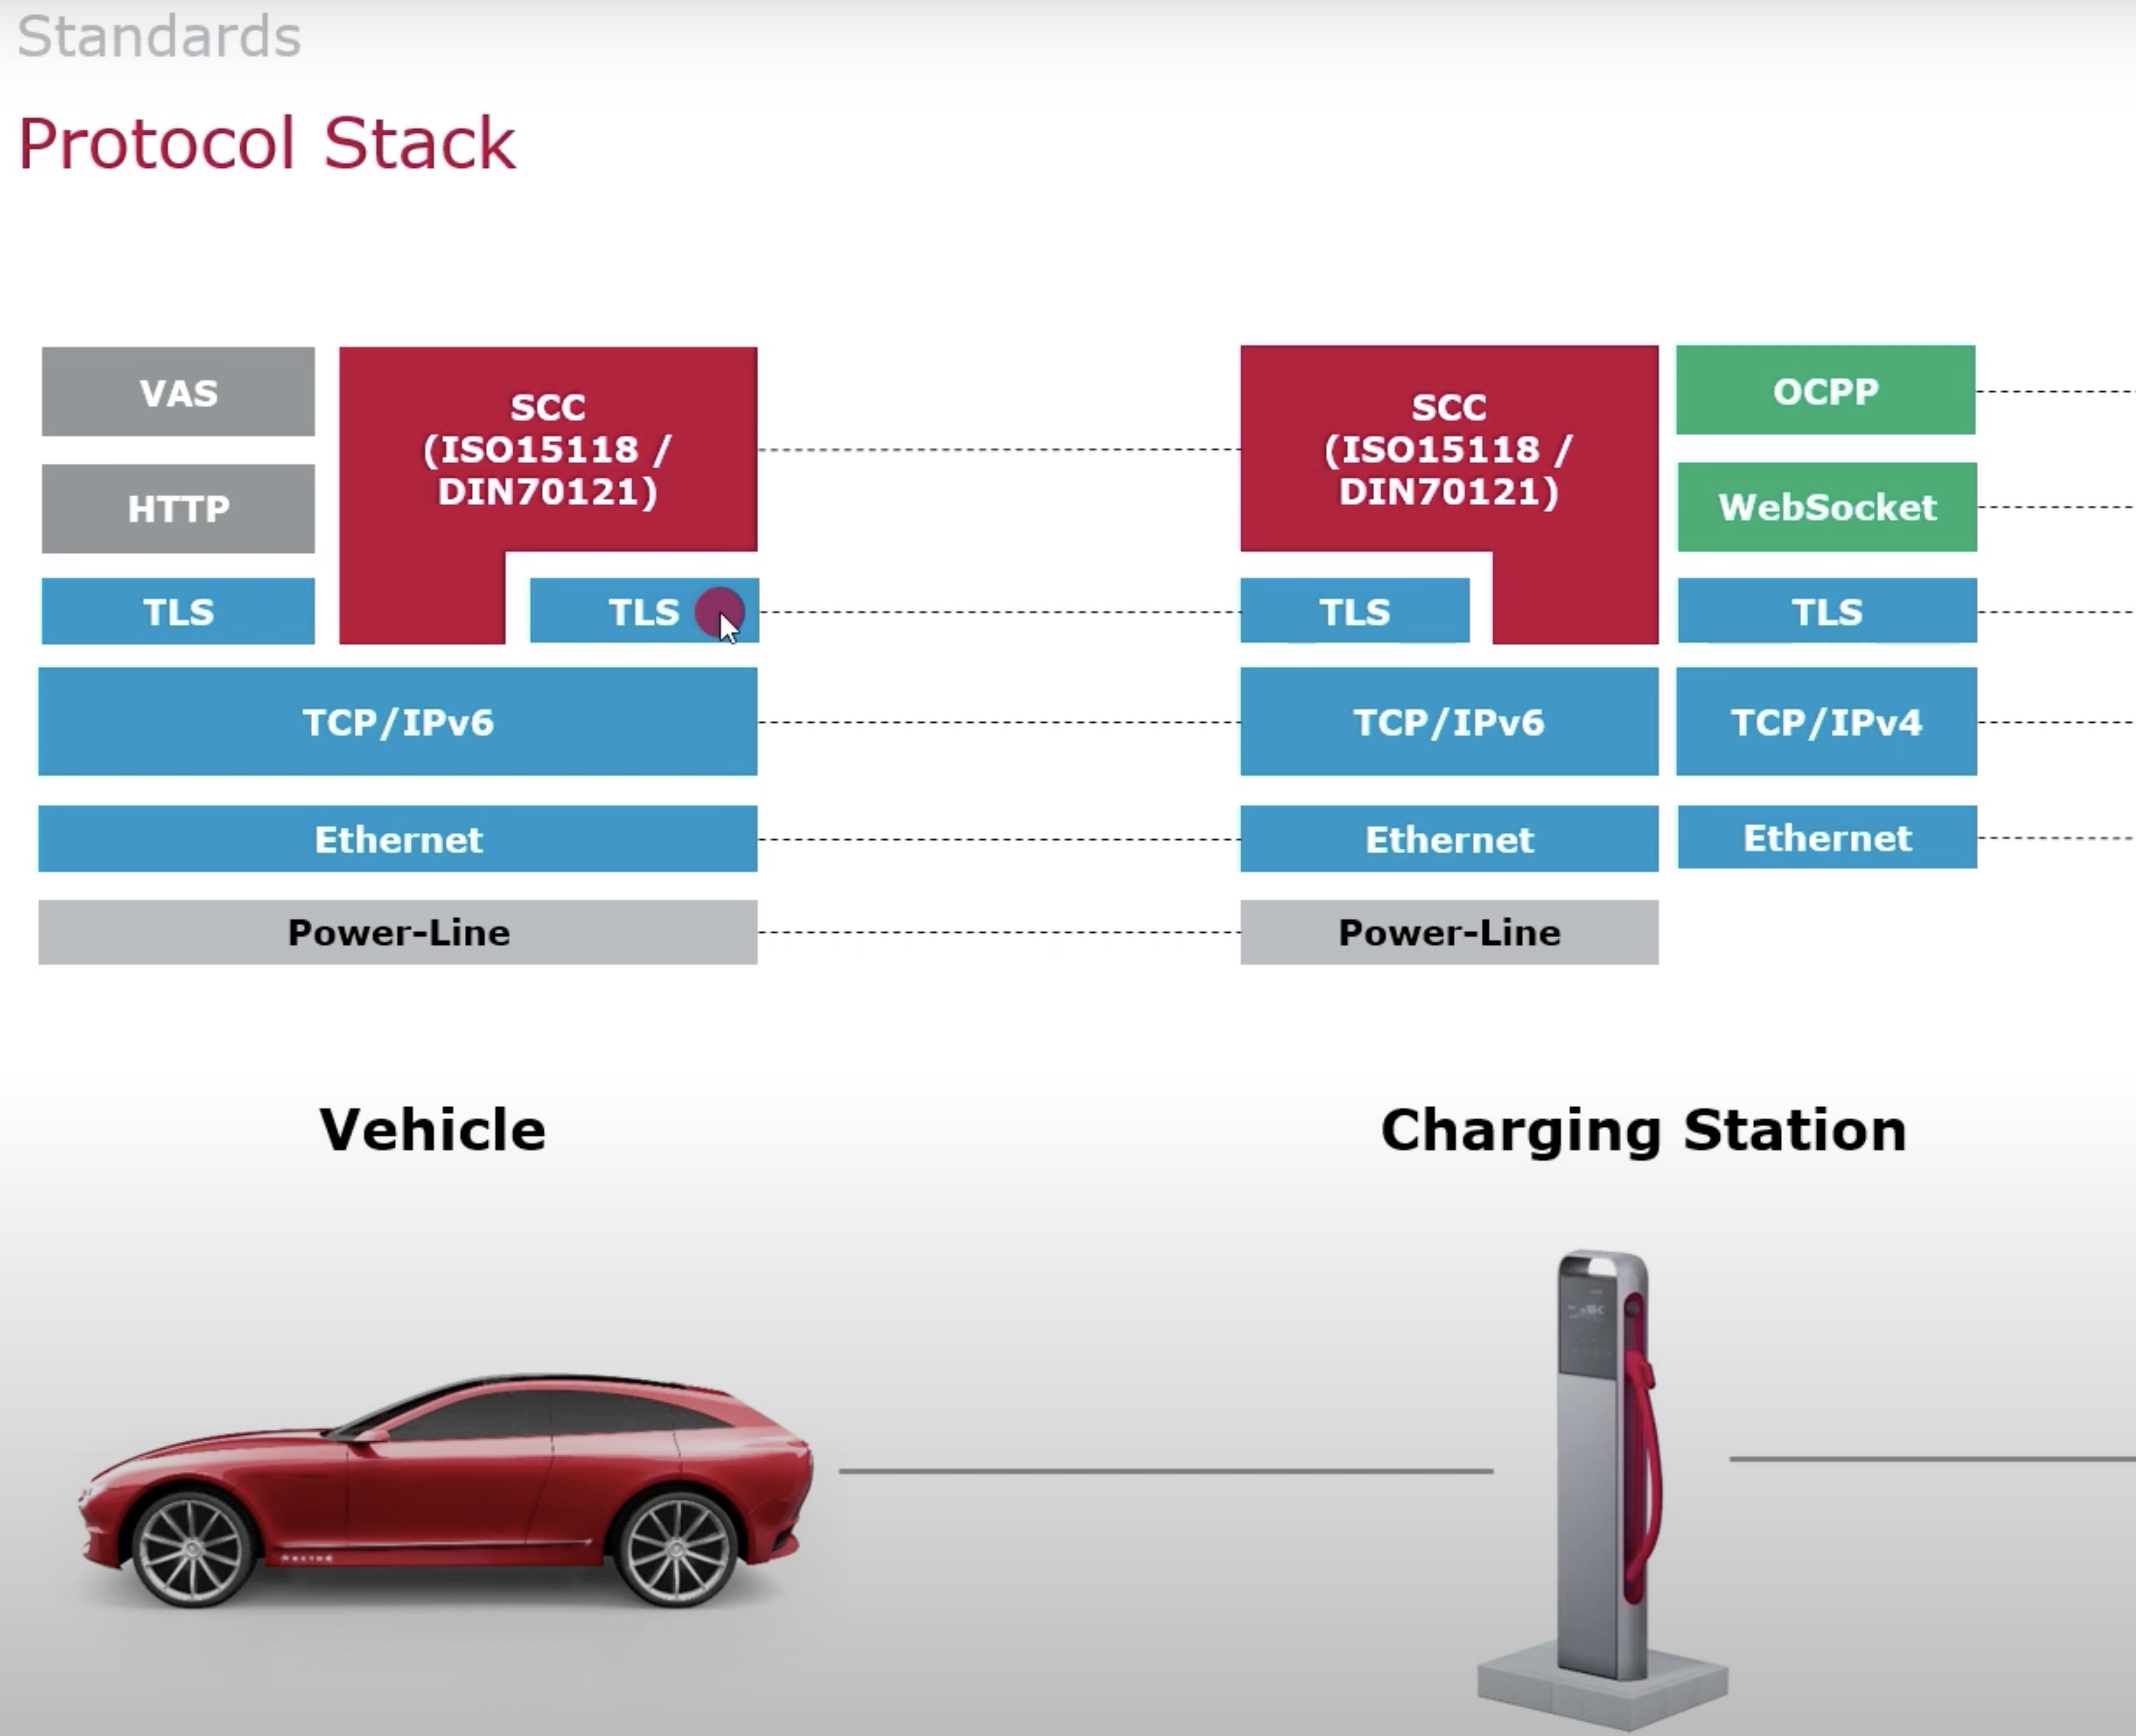
\includegraphics[width=0.6\linewidth]{images/EV_CS_Protocols.png}
    \caption[Current Electric Vehicle and Charging Station protocols]{Current Electric Vehicle and Charging Station protocols \protect \footnotemark}
    \label{fig:ev_cs_protocols}
\end{figure}

\footnotetext{\url{https://www.youtube.com/watch?v=S\_llUuyAcqs}}

\subsection{Evaluation of the General Architecture of SSI with IoT}
\label{subsec:evaluation_of_the_general_architecture}

It was evident that the Verifiable Electric Vehicle Charging System as proposed in this work is able to fulfill most of the requirements, with the ones that were not having been provided documentation in order to apply them in the future.

Despite having presented one use case of Self-Sovereign Identity with Internet of Things devices (EVs and CSs) that presents good prospects for adoption, assessing the general architecture presented on Section~\ref{subsec:architecture_for_ssi_with_iot} requires a more in-depth analysis, making use of other case studies. For this end, more use cases need to be discussed to give power to this idea. Nonetheless, it was possible to verify that in IoT devices that do not lack computational power and electricity, there are existing implementations of agents and networks that could be used by such devices, like an EV. On top of that, the general architecture presents the necessary components for any Self-Sovereign Identity system that has agents acting on behalf of any entity, whether humans, organizations, or IoT devices.

